\documentclass{article}
\usepackage{graphicx}
\usepackage{amsmath}
\usepackage{listings}
\usepackage{url}
\title{Project 13 - Two-sided Jacobi algorithm for SVD}
\author{Thomas Toft Lindkvist - 201905635 - AU643642}
\date{}
\begin{document}
    \maketitle
    Since my student number ends with 35, I have been tasked with project $ 35 \mod 22 = 13 $.
    My repository, wherein the examination project lies, can be found at \url{https://github.com/ttlindkvist/ppnm/} .
    I have done testing to ensure correctness and timed the algorithm to visualize the $ O(n^3) $ operational cost.
    
    \section{Elementary Jacobi diagonalization}
    As we know we can use Jacobi rotations to diagonalize a real symmetric matrix $ A $ into
    \begin{align}
    	A = VDV^T
    \end{align}
	This can be done by sweeping across the upper triangle of the matrix cyclically, eliminating off-diagonal elements one-by-one, by a well-tuned Jacobi rotation $ J(p,q) $ eliminating element $ A_{pq}=A_{qp} $.
	\begin{align}
		A \to A' = J(p,q)^T A J(p,q)
	\end{align}
	
	But what if we want to find the singular values of a non-symmetric, square matrix? Can we reuse some of what we know from this method? It turns out the answer is yes! But first what is SVD.
	
	\section{SVD}
	The singular value decomposition (SVD) of a matrix $ A $ is a factorization of the matrix on the form
	\begin{align}
		A = UDV^T,
	\end{align}
	where $ U $ and $ V $ are orthogonal matrices and $ D $ is a diagonal matrix containing the singular values of $ A $. These \textit{singular values} are the square roots of the eigenvalues of the real symmetric matrix $ A^TA $.	
	
    
    \section{Two-sided Jacobi method}
    Many parts of the Jacobi algorithm for the symmetric case can be reused! 
    \subsection{Square matrices}
    In fact the only modification necessary 
    
    TODO: PROOF than the Givens angle is what it is!
    
    \subsection{Tall matrices}
    For tall matrices $ A $ of size $ N\times M $, $ N\geq M $, a small adjustment has to be made. First a QR-factorization is necessary, and is done using my own Gram-Schmidt implementation from a homework
    \begin{align}
    	A=QR.
    \end{align}
    Since R now is a square matrix, we can use the above method for generating a SVD for R
    \begin{align}
    	R = U'DV^T.
    \end{align}
	So we can write $ A $ as
	\begin{align}
		A = Q(U'DV^T),
	\end{align}
	which is almost the SVD. But since the product of two orthogonal matrices is also! an orthogonal matrix, the SVD for $ A $ is simply
	\begin{align}
		A = UDV^T,\quad U = QU'.
	\end{align}
    
    \section{Testing}
    How do we prove that the method works? As seen from the output (see github), it works for small matrices by visual inspection, but we could just be lucky.
    
    Testing is done by generating a bunch of large, tall matrices, and checking if the resulting $ U $ and $ V $ are orthogonal (by checking $ U^TU $ and $ V^TV $ is identity), and by checking that $ D $ is diagonal. Then, by definition, the algorithm must be producing the correct output. 
    
    \section{Computational cost}
    Just as the algorithm for symmetric matrices, the cyclic method for SVD is an $ O(n^3) $ operation as seen on figure \ref{fig:timing}. A fit to the time taken to SVD different sized random square matrices, shows the $ O(n^3) $ cost.
    What is also seen is a comparison with the GSL implementation of a one-sided Jacobi algorithm - which is around 8-11 times faster in these use-cases.
    \begin{figure}
    	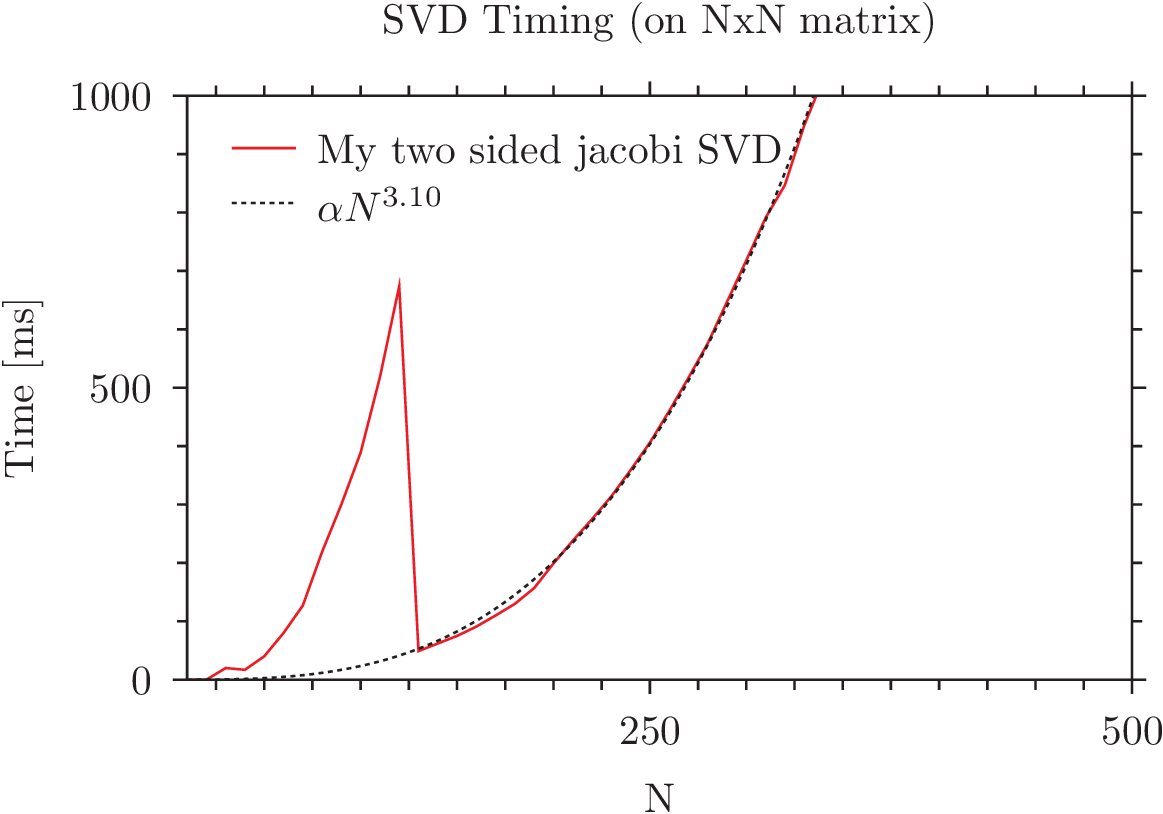
\includegraphics{timing.png}
    	\caption{Timing of my implementation of the two sided Jacobi SVD versus the GSL implementation of the one-sided Jacobi SVD on random N by N matrices.}
    	\label{fig:timing}
    \end{figure}
    
    
    
\end{document}